

\chapter{An Outline of the Quantum Field Theory of the Standard Model}
\label{sec:physics:qft}


Quantum Field Theory combines special relativity and quantum mechanics to describe the Lorentz invariant rules for fields representing particles and forces. The foundation of QFT is the principle of least action.
\begin{equation}
    \delta s = \delta \int \mathcal{L}(\phi, \partial_\mu \phi) dx = 0,
    \label{eqn:physics:qft:leastAction}
\end{equation}

\noindent which leads to the Euler-Lagrange equation of motion for the fields:
\begin{equation}
    \frac{\partial}{\partial x_\mu} \bigg( \frac{\partial \mathcal{L}}{\partial(\partial \phi / \partial x_\mu)}\bigg) - \frac{\partial \mathcal{L}}{ \partial \phi} = 0,
    \label{eqn:physics:qft:lagrangeEoM}
\end{equation}

\noindent where $\mathcal{L}(\phi, \partial_\mu \phi)$ is the Lagrangian of the quantum fields. In such a framework, the behaviors of the quantum fields are then fully dictated by their Lagrangian via the Euler-Lagrangian Equation of Motion in Equation~\ref{eqn:physics:qft:lagrangeEoM}. Therefore, this allows us to encode our understanding of the dynamics and interactions of field into the Lagrangian. For example, Klein-Gordon Equations and Dirac Equations, which are two versions of the generalization of Schrodinger Equation in the special relativity domain, can be derived from the Lagrangian of the massive scalar field $\phi$ and massive spinor filed $\psi$, as shown in Equation~\ref{eqn:physics:qft:kleinGorden} and \ref{eqn:physics:qft:dirac}. Another example is the electromagnetic field. Based on the Gauss's Law $\nabla \cdot \vec{E} = 0$ and $\nabla \cdot \vec{B} = 0$, Faraday's law of induction $\nabla \times \vec{E} = - \partial_t \vec{B}$ and Ampere's circuital law $\nabla \times \vec{B} = (1/c) \partial_t \vec{E}$, the Maxwell equations for electromagnetic field in the free space can be achieved by defining a Lagrangian of a massless vector field $A_\mu$, as shown in Equation~\ref{eqn:physics:qft:maxwell}.
\begin{align}
    \text{scalar:} \,
    \mathcal{L}_\phi &= \frac{1}{2} \partial_\mu\phi \partial^\mu \phi - \frac{1}{2} m^2 \phi^2 
        &\Longrightarrow& \;  \text{ Klein-Gordon Equation:} \, \partial_\mu \partial^\mu \phi + m^2 \phi = 0 \label{eqn:physics:qft:kleinGorden}\\
    \text{spinor:} \,
    \mathcal{L}_\psi &= i \bar{\psi}\gamma^\mu \partial_\mu \psi - m \bar{\psi} \psi 
        &\Longrightarrow& \; \text{ Dirac Equation:}  \, (i\gamma^\mu\partial_\mu - m) \psi = 0 \label{eqn:physics:qft:dirac} \\
    \text{vector:} \,
    \mathcal{L}_A &= -\frac{1}{4}F_{\mu\nu} F^{\mu \nu} 
        &\Longrightarrow& \; \text{ Maxwell Equations:} \, \partial_\mu \partial^\mu A_\mu = 0 \label{eqn:physics:qft:maxwell}
\end{align}


The first well-established quantum field theory is Quantum Electrodynamics (QED). Its formulation in the early 20th century was a joint effort from many great physicists such as Paul Dirac, Wolfgang Pauli, Werner Heisenberg, and Enrico Fermi. Since its establishment, QED was able to successfully explain many atomic phenomena that involve photon and charged particles, such as spontaneous photon emission in the atoms. However, in the late 1930s, physicists realized that QED calculation could diverge during the next-to-leading order. This causes skepticism to QED to make meaningful predictions when involving loops. This problem was solved by proving that the divergence in the fermion vacuum polarization and interaction vertices can exactly cancel out each other. Therefore QED is renormalizable. 1965 Nobel Prize in Physics was awarded to Shinichiro Tomonaga, Julian Schwinger, and Richard Feynman for their contributions to the QED renormalization. SM is an extension based on QED, which extends the gauge symmetry in QED from $U(1)$ to $U(1)_Y \times SU(2)_L \times SU(3)_c$, including electroweak and strong force. Several milestones along the establishment of SM involves

\begin{itemize}
    \item \textbf{Yang-Mills Theory.} In 1954, Chen-Ning Yang and Robert Mills described the gauge theory for the non-abelian group \cite{PhysRev.96.191}. It serves as one of the most impotent theoretical frameworks for SM. Based on Yang-Mills Theory, SM QCD is developed and Electroweak force is unified. 
    
    \item \textbf{Higgs mechanism.} In 1964, the Higgs mechanism to generate the mass of gauge field via spontaneous symmetry breaking was proposed by three independent groups: Robert Brout and François Englert \cite{PhysRevLett.13.321}; by Peter Higgs \cite{PhysRevLett.13.508}; and by Gerald Guralnik, C. R. Hagen, and Tom Kibble \cite{PhysRevLett.13.585}. 
    
    \item \textbf{GWS Model.} In 1961 Gheldon Glashow combines the electromagnetic and weak force based on Yang-Mills gauge field \cite{Glashow:1961tr}; then in 1967, Steven Weinberg and Abdus Salam incorporated the Higgs Mechanism into Glashow's electroweak theory \cite{PhysRevLett.19.1264}. In 1972, the massive Yang-mills gauge fields with gauge boson mass generated by the Higgs mechanism is proven renormalizable by Gerard 't Hooft and Martinus Veltman \cite{tHooft:1972tcz}. In 1973, CKM matrix was added to GWS theory to allow quark mixing and CP violation.
    
    \item \textbf{Quark Model and QCD.} In 1964, the quark model was proposed by Murray Gell-Mann in order to classify a increasing number of newly discovered mesons and baryons. Quark model soon obtained supports from experiments, such as deep inelastic scattering experiments at SLAC starting in 1969, the discoveries of $J/\psi (c\bar{c})$ at Brookhaven National Laboratory and SLAC in 1974, Ubsilon $\Upsilon (b\bar{b})$ at Fermilab in 1977, and top quark at Fermilab in 1995.  In 1973, asymptotic freedom was proposed by David Gross and Frank Wilczek, and independently by David Politzer, to explain the quark confinement: strong interaction allows perturbation calculation at high energy while confined at low energy.
\end{itemize}

This section gives a brief summery of SM skeleton in aspect of the Yang-Mills theory, higgs mechanism, GWS Theory, Quark asymptotic freedom in QCD. Before starting, we may remind ourselves the final form of the SM Lagrangian:

\begin{equation}
\begin{split}
    \mathcal{L}_{U(1)\times SU(2) \times SU(3)} =&   - \frac{1}{4}B_{\mu\nu}B^{\mu\nu} - \frac{1}{4}W^a_{\mu\nu}W^{\mu\nu}_a - \frac{1}{4}G^a_{\mu\nu}G^{\mu\nu}_a\\
    & + \bar{\chi}_L \gamma^\mu \big( i \partial_\mu -g \frac{\tau_a}{2} W^a_\mu -g'\frac{Y}{2} B_\mu \big) \chi_L 
    + \bar{\psi}_R \gamma^\mu \big( i \partial_\mu -g'\frac{Y}{2} B_\mu \big) \psi_R 
    - g_s (\bar{q}\gamma^\mu  T_{a} q) G_\mu^a \\
    & + \left\lvert  \big( i \partial_\mu -g \frac{\tau_a}{2} W^a_\mu -g'\frac{Y}{2} B_\mu \big)\phi \right\rvert ^2 - V(\phi) \\
    & -(y_1 \bar{\chi}_L \phi \psi_R + y_2 \bar{\chi}_L \phi_c \psi_R + \text{hermitian conjugate}),
\end{split}
\label{eqn:physics:qft:smLagrangian} 
\end{equation}

\noindent where the first to the forth row represents the gauge sector, fermion sector, higgs sector and fermion mass sector respectively. This total SM Lagrangian functions as an indexing map of the discussion in this section. One of the beauty of SM is its minimality. We can count the number of free parameters in the SM Lagrangian. Thanks to the symmetries imposed in the SM, only 18 basic free parameters to begin with are needed in the model.
\begin{itemize}
    \item 3 gauge coupling strength for hypercharge, isospin and color. $g$, $g'$, $g_s$.
    \item 2 parameters $\mu$ and $\lambda$ in the higgs potential field $V(\phi)=\frac{1}{2} \mu^2 \bar{\phi}\phi + \frac{1}{4} \lambda(\bar{\phi}\phi )^2 $
    \item 9 Yukawa couplings between higgs and 9 charged fermions: $y_e$,$y_\mu$,$y_\tau$,$y_u$,$y_d$,$y_c$,$y_s$,$y_t$,$y_b$
    \item 4 parameters in the CKM matrix, 3 Euler angles $\theta_{12}$, $\theta_{23}$, $\theta_{23}$ and CP violating phase $\delta$.
\end{itemize}

The values of these free SM parameters are determined from the experiments. In addition to the above 18 basic parameters, neutrino oscillation indicates neutrinos are not massless and their flavor eigenstates are a mixing of the mass eigenstates. Accordingly, three additional Yukawa couplings are needed for neutrino mass. Analogical to the CKM matrix for the quark mixing, the neutrino mixing is described by PMNS matrix which has 4 free parameters corresponding to three rotation angles and a CP violation phase. Moreover, the CP violation in QCD could also be allowed by adding an extra parameter $\delta_{CP}$. However, in the experiment, the QCD CP violation is not observed in contrast with the considerable CP violation observed in the weak interaction. This CP conservation in QCD is often referred to as "strong CP problem". So $\delta_{CP}$ could be treated as a free SM parameter with a very small value yet to be measured.



%  The Standard Model of particle physics is is a quantum field theory which is gauge sysmmetric. In 1920s, Dirac 


% With a set of amazing theoretical achievements and experimental discoveries since 1900s, we come to the modern understanding of particles physics, the Standard Model. The milestone achievements alone the path includes but not limited to the Yang-Mills theory, the spontaneous symmetry breaking and higgs mechanism, the GWS electroweak theory, the quark model, the renormalization of EW and QCD.  the P violation in Weak interaction, the CP violation in K meson decay, the discovery on WZ boson at CERN, the ,  Perhaps, the SM is the most ultimate answer the humanity have devised so far to the question of "what is the world made of". 







\section{Gauge Symmetry}
\label{sec:physics:qft:gaugeSymmetry}

Gauge theory is a type of quantum field theory, the Lagrangian of which is invariant under local phase transformations or gauge transformations. The term ``gauge" should be understood as the regularization of the redundant degrees of freedom in the Lagrangian. The transformations between different gauges form a Lie group, which characterizes this gauge theory. Yang-Mills gauge theory is the gauge theory for the non-abelian Lie groups. (``abelian" or ``non-abelian" tells whether two gauge transformations in the group are commutable or not.) The standard model is built based on the Yang-Mills gauge theory. But why does SM have to respect the gauge symmetry? The primordial reason is that by enhancing the global phase symmetry to local phase symmetry, we can introduce massless gauge bosons and consequently obtain the couplings between the fermions and the gauge boson. Another benefit anchors in the renormalization. A QFT is useful only if it is renormalizable to make finite meaningful predictions. And gauge theory is proven renormalizable. Besides obtaining force and renormalization, a relatively modern understanding of gauge symmetry is that it is not a symmetry in nature but an artificial consequence of the redundant degree of freedom in the theory. According to Noether's theorem, a nature symmetry corresponds to a conservation law. For example, the global gauge symmetry of QED gives rise to the conservation of electric charge. But the local symmetry in the QED, which is related to the redundant degree of freedom in the mathematical description of the photo polarization, does not lead to any corresponding conserved current. The thinking about the essence of the gauge symmetry is nicely presented in Schwartz's book, \textit{Quantum Field Theory and the Standard Model} \cite{schwartz2014quantum}. Here provide a description of the gauge symmetry of the abelian U(1) group and the non-abelian SU(2), SU(3) groups, which is crucial for SM electroweak and QCD, as well as beyond SM models for lepton non-universality in Section~\ref{sec:physics:bsm}.


\subsection{U(1) Gauge Symmetry}
The Lagrangian of a U(1) gauge theory with spinnor field $\psi$ and the associated gauge vector field $B_\mu$ is
% 
\begin{equation}
    \mathcal{L}_{U(1)} = i\bar{\psi}\gamma^\mu D_\mu \psi  - m\bar{\psi} \psi  - \frac{1}{4}B_{\mu\nu}B^{\mu\nu},
    \label{eqn:physics:qft:u1Lagrangian}
\end{equation}

\noindent where the covariant derivative $D_\mu$ and covariant field strength tensor $B_{\mu\nu}$ defined as
% 
\begin{equation}
    D_\mu \equiv \partial_\mu +i g' \frac{Y}{2} B_\mu , \;\;\; 
    B_{\mu\nu} \equiv  \partial_\mu B_\nu - \partial_\nu B_\mu.
\end{equation}

\noindent $\mathcal{L}_{U(1)}$ is invariant under U(1) local transformation
% 
\begin{equation}
	\psi \longmapsto e^{i\alpha(x_\mu)} \psi ,\;\;\; 
	B_\mu  \longmapsto  B_\mu - \frac{1}{g'\frac{Y}{2}}\partial_\mu \alpha(x_\mu).
\end{equation}

\noindent The interaction between the U(1) charge current $j^\mu \equiv g' \bar{\psi}\gamma^\mu \psi$ and the gauge field $B_\mu$ is $-j^\mu A_\mu$ and is embedded in the covariant derivative $D_\mu$. The QED is a U(1) Gauge theory. So the QED Lagrangian takes the form of equation~\ref{eqn:physics:qft:u1Lagrangian}. If we choose $g'\frac{Y}{2} = -e$ and use the conventional notation $A_\mu$ for the QED gauge field, equation~\ref{eqn:physics:qft:u1Lagrangian} becomes the common form of QED Lagrangian.


\subsection{SU(2) Gauge Symmetry}

The three generators of SU(2) group $T_a$ with $a \in {1,2,3 }$ are usually represented by the half of Pauli Matrices $T_a = \frac{1}{2} \tau_a = \frac{1}{2} \sigma_a$, where the Pauli Matrices are 
%
\begin{equation}
    \sigma_1 = \begin{bmatrix} 0 & 1 \\ 1 & 0\end{bmatrix}, \;\;\; 
    \sigma_2 = \begin{bmatrix} 0 & -i \\ i & 0\end{bmatrix}, \;\;\; 
    \sigma_3 = \begin{bmatrix} 1 & 0 \\ 0 & -1\end{bmatrix}.
\end{equation}

\noindent The commutation relation of the group generators can be represented as $[T_a, T_b] = i f_{abc} T_c$, where $f_{abc}$ is the structure constant of the group. For SU(2) group, the structure constant is the Levi-Civita symbol $f_{abc}=\epsilon_{abc}$. In SM, the left-handed neutrino and charged lepton in the same generation form a doublets described by $SU(2)$ group. The same scenario is for the up and down type left-handed quark in the same generation. The higgs doublet in the SM also transforms as a global $SU(2)$ group. Other than the applications in the SM, SU(2) group is also useful in the description of nucleons with proton-neutron doublet $[n, p]$. 

\noindent Now we consider a SU(2) gauge theory. Suppose there are two spinor fields $\psi_1$ and $\psi_2$, which compose a spinor doublet $\chi = [ \psi_1, \psi_2 ]^T$. the Lagrangian of the spinnor doublet $\chi$ and the gauge vector triplet $W^a$ is
%
\begin{equation}
\begin{split}
    \mathcal{L}_{SU(2)}  &= (i\bar{\psi}_1\gamma^\mu D_\mu \psi_1  - m_1\bar{\psi_1} \psi_1) + (i\bar{\psi}_2\gamma^\mu D_\mu \psi_2  - m_2\bar{\psi_2} \psi_2)  - \frac{1}{4}W^a_{\mu\nu}W^{\mu\nu}_a \\
    &= i\bar{\chi}\gamma^\mu D_\mu \chi  - m\bar{\chi} \chi  - \frac{1}{4}W^a_{\mu\nu}W^{\mu\nu}_a,
\end{split}
\label{eqn:physics:qft:su2Lagrangian}
\end{equation}

\noindent where the covariant derivative $D_\mu$ and covariant field strength tensor $W^a_{\mu\nu}$ defined as
%
\begin{equation}
    D_\mu \equiv \partial_\mu +i g \frac{\tau_a}{2} W^a_\mu , \;\;\; 
    W^a_{\mu\nu} \equiv  \partial_\mu W^a_\nu - \partial_\nu W^a_\mu - g f_{abc} W^b_\mu W^c_\nu
\end{equation}

\noindent $\mathcal{L}_{SU(2)}$ is invariant under SU(2) local transformation 
%
\begin{equation}
	\chi \longmapsto  e^{i\alpha^a (x_\mu) \frac{\tau_a}{2}} \chi , \;\;\; 
    W^a_\mu \longmapsto  W^a_\mu - \frac{1}{g}\partial_\mu \alpha^a(x_\mu) - f_{abc}\alpha^b(x_\mu) W^c_\mu 
\end{equation}

\noindent Because SU(2) group is non-abelian, the nontrivial group structure $f_{abc}$ has its contribution to the covariant field strength tensor $W^a_{\mu\nu}$. This leads to the fact that the term $\frac{1}{4}W^a_{\mu\nu}W^{\mu\nu}_a$ in the equation~\ref{eqn:physics:qft:su2Lagrangian} not only involves the kinetic energy of the gauge field but also includes $WWW$ and $WWWW$ terms representing three points and four-point self-interaction of the gauge field. The gauge boson can self interact when gauge symmetry is imposed on a non-abelian group, a unique feature of the non-abelian gauge theories. As we will see in the GWS theory in Section~\ref{sec:physics:qft:gws}, this leads to the Triple-Gauge-Coupling (TGC) and Quatic-gauge-coupling (QGC) in the SM.




\subsection{SU(3) Gauge Symmetry}
The eight generators of SU(3) group $T_a$ with $a \in {1,2,\dots 8}$ are usually represented by the half of Gell-mann Matrices $T_a = \frac{1}{2} \lambda_a$, where the Gell-mann Matrices are 
%
\begin{equation}
\begin{split}
    \lambda_1 &= \begin{bmatrix} 0 & 1 & 0 \\ 1 & 0 & 0 \\ 0 & 0 & 0\end{bmatrix}, \;\;\; 
    \lambda_2 = \begin{bmatrix} 0 &-i & 0 \\ i & 0 & 0 \\ 0 & 0 & 0\end{bmatrix}, \;\;\; 
    \lambda_3 = \begin{bmatrix} 1 & 0 & 0 \\ 0 &-1 & 0 \\ 0 & 0 & 0\end{bmatrix}, \;\;\; 
    \lambda_8 = \begin{bmatrix} 1 & 0 & 0 \\ 0 & 1 & 0 \\ 0 & 0 &-2\end{bmatrix}, \\
    %
    \lambda_4 &= \begin{bmatrix} 0 & 0 & 1 \\ 0 & 0 & 0 \\ 1 & 0 & 0\end{bmatrix}, \;\;\; 
    \lambda_5 = \begin{bmatrix} 0 & 0 &-i \\ 0 & 0 & 0 \\ i & 0 & 0\end{bmatrix}, \;\;\; 
    \lambda_6 = \begin{bmatrix} 0 & 0 & 0 \\ 0 & 0 & 1 \\ 0 & 1 & 0\end{bmatrix}, \;\;\; 
    \lambda_7 = \begin{bmatrix} 0 & 0 & 0 \\ 0 & 0 &-i \\ 0 & i & 0\end{bmatrix}.
\end{split}
\end{equation}

\noindent The SU(3) group has non-trivial structure constants which are $f_{123}=1, f_{147}= f_{246}=f_{257}= f_{345}= f_{516}= f_{637}=\frac{1}{2}, f_{458} = f_{678}=\frac{\sqrt{3}}{2}$. Besides the structure constant $f_{abc}$, there are also three useful group constants $T_R, C_F, C_A$ defined as below, with their values for SU(3) group on the right side
%
\begin{align}
	Tr(T^aT^b)=T_R \delta^{ab}  &\longrightarrow  T_R^{SU(3)}  = \frac{1}{2} \\
    T_a^{i,k}T^a_{k,j} = C_F \delta_{ij}  &\longrightarrow  C_F^{SU(3)} = \frac{N_c^2-1}{2N_c} = \frac{4}{3} \\
    f_{acd}f^{bcd} = C_A \delta_{ab} &\longrightarrow C_A^{SU(3)}  =N_c = 3
\end{align}

\noindent where $N_c$ is the number of charges or colors. These constants often appear in the calculation of the renormalization of the group. In the SM, SU(3) group is used to describe the triplet of three colors $r,g,b$ in the QCD. In addition to the application in SM, SU(3) group is also useful to describe light mesons and baryons which consist of $[u,d,s]$ quarks. For light mesons, two light quarks form $SU(3) \times SU(3)$ group, while for light baryon, three light quarks form $SU(3) \times SU(3) \times SU(3)$ group.


\noindent Now we consider SU(3) gauge theory. Suppose there are three spinor fields $\psi_r$, $\psi_g$, $\psi_b$, which compose a spinor triplet $q = [ \psi_r, \psi_g, \psi_b ]^T$. Lagrangian of the spinnor triplet $q$ and the gauge field octolet $G^a$ is
\begin{equation}
\begin{split}
    \mathcal{L}_{SU(3)}  &= \sum_{k \in \{r,g,b\}} \big( i\bar{\psi_k}\gamma^\mu D_\mu \psi_k  - m\bar{\psi_k} \psi_k \big) - \frac{1}{4}G^a_{\mu\nu}G^{\mu\nu}_a \\
    &= i\bar{q}\gamma^\mu D_\mu q  - m\bar{q} q - \frac{1}{4}G^a_{\mu\nu}G^{\mu\nu}_a
\end{split}
\label{eqn:physics:qft:su3Lagrangian}
\end{equation}

\noindent where the covariant derivative $D_\mu$ and covariant field strength tensor $G^a_{\mu\nu}$ defined as
\begin{equation}
    D_\mu \equiv \partial_\mu +i g T_a G^a_\mu , \;\;\; 
    G^a_{\mu\nu} \equiv \partial_\mu G^a_\nu - \partial_\nu G^a_\mu - g_s f_{abc} G^b_\mu G^c_\nu
    \label{eqn:physics:qft:su3Covariant}
\end{equation}

\noindent $\mathcal{L}_{SU(3)}$ is invariant under SU(3) local transformation 
\begin{equation}
	q \longmapsto  e^{i\alpha_a (x_\mu) T^a} q , \;\;\; 
    G^a_\mu \longmapsto  G^a_\mu - \frac{1}{g''}\partial_\mu \alpha^a(x_\mu) - f_{abc}\alpha^b(x_\mu) G^c_\mu 
\end{equation}



\noindent The same as the $SU(2)$  scenario, the covariant field strength tensor $G^a_{\mu\nu}$ in Equation~\ref{eqn:physics:qft:su3Covariant}  has contributions from the non-trivial group structure $f_{abc}$ of $SU(3)$ group, so the kinematic term of gauge field $\frac{1}{4}G^a_{\mu\nu}G^{\mu\nu}_a$ in the Lagrangian in Equation~\ref{eqn:physics:qft:su3Lagrangian} not only involves the kinematic energy of the gauge field but also include $GGG$ and $GGGG$ terms representing the three-point and four-point self-interaction of the gauge field. For QCD in SM, gluon's self-interaction leads to many unique phenomenologies in the strong interactions, such as quark confinement, evolution of the parton distribution functions and final state ration, which will be discussed in Section~\ref{sec:physics:qft:qcd}.





\section{The Higgs Mechanism}
\label{sec:physics:qft:higgsMechanism}
One might notice that the gauge fields discussed above in Section~\ref{sec:physics:qft:gaugeSymmetry} are all massless: the Lagrangians do not have any terms for the gauge fields' mass because directly adding such mass terms breaks the gauge symmetry. The massless gauge field does not cause problems in the QED and QCD, where photon and gluon are indeed massless. But for weak interaction, it is known that weak force is short-range, and thus the weak bosons must be massive. But if we naively add a mass term for the weak boson by hand, e.g. $m W_\mu W^\mu$, and give up the gauge symmetry, we will come across divergence in the loop integrals related to the propagator and end up with an un-renormalizable theory failing to make any meaningful predictions at high energy scale. The way to get around is the ``higgs mechanism" which generates mass for gauge bosons via spontaneous symmetry breaking while maintaining the gauge symmetry. It first introduces a scalar field $\phi$ with spontaneously-broken global symmetry. $\phi$ has gauge charge, and thus couples via the covariant derivative with the gauge filed that desires mass. Eventually, it is the gauge covariant derivatives of a spontaneously-broken $\phi$ that provides the mass for the gauge field. For this reason, the mass of the gauge particle is often intuitively interpreted as the ``resistance" when the gauge boson moves in the $\phi$ field and interacts with it. In this subsection, the higgs mechanism with $U(1)$ and $SU(2)$ spontaneously broken symmetry are illustrated.

\begin{figure}[ht]
    \centering
    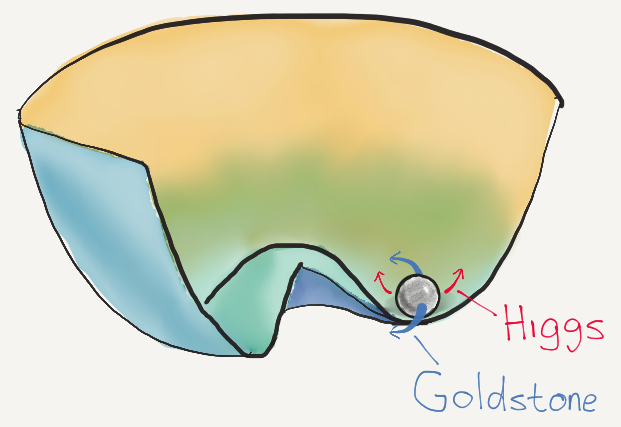
\includegraphics[width=0.5\textwidth]{chapters/Physics/sectionQFT/figures/Higgs.png}
    \caption{Spontaneous symmetry breaking of the scalar field $\phi$  with a $U(1)$  global symmetric potential. The shape of potential on the complex plane looks like a Mexican hat. The scalar field's minimum potential shifts from the origin by the amount of Higgs vacuum expectation value, forming a ring of positions with minimal potential. The scalar field has to choose one of the positions on the ring to settle down. Such a choice is so-called spontaneous symmetry breaking. The radial and lateral perturbation mode around this minimal position gives rise to the Higgs field and the Goldstone field. }
    \label{fig:physics:qft:higgsPotential}
\end{figure}



\subsection{U(1) SSB}

Consider a $U(1)$ gauge theory with a scalar field $\phi$, which has a $U(1)$ global symmetric potential
\begin{equation}
    V(\phi) = \frac{1}{2} \mu^2 \phi^*\phi + \frac{1}{4}\lambda(\phi^*\phi )^2.
\end{equation}


\noindent When engaging local symmetry, we introduce the associated gauge field $B_{\mu}$. The total Lagrangian for the scalar field and the gauge field is
\begin{equation}
\begin{split}
	\mathcal{L} & = D^\mu\phi^* D_\mu\phi-V(\phi)   - \frac{1}{4}B_{\mu\nu}B^{\mu\nu} \\
	& = D^\mu\phi^* D_\mu\phi- \big(\frac{1}{2} \mu^2 \phi^*\phi + \frac{1}{4} \lambda(\phi^*\phi )^2 \big)   - \frac{1}{4}B_{\mu\nu}B^{\mu\nu},
\end{split}
\label{eqn:physics:qft:u1Higgs}
\end{equation}

\noindent where the covariant derivative $D_\mu$ and covariant field strength tensor $B_{\mu\nu}$ defined as
\begin{equation}
    D_\mu \equiv \partial_\mu +i g' \frac{Y}{2} B_\mu ,\;\;\; 
    B_{\mu\nu} \equiv  \partial_\mu B_\nu - \partial_\nu B_\mu,
\end{equation}

\noindent and the gauge transformation of the scalar field and gauge field is
\begin{equation}
	\phi \longmapsto e^{i\alpha(x_\mu)} \phi ,\;\;\; 
	B_\mu  \longmapsto  B_\mu - \frac{1}{g'\frac{Y}{2}}\partial_\mu \alpha(x_\mu).
    \label{eqn:physics:qft:u1HiggsGaugeTransform}
\end{equation}


\noindent The Lagrangian in Equation~\label{eqn:physics:qft:u1Higgs} is invariant under $U(1)$ gauge transformation in Equation~\label{eqn:physics:qft:u1HiggsGaugeTransform}. At this moment, $B_\mu$ is massless. The spontaneous symmetry breaking is concerning the scalar's potential $V(\phi)$. When $\mu^2<0$ , the scalar field's potential $V(\phi)$ on the complex plane looks like a Mexican hat, shown in Figure~\ref{fig:physics:qft:higgsPotential}. It has an infinite number of positions with minimal potential on a ring with $|\phi|^2 = -\frac{\mu^2}{\lambda} = \nu^2$, where $\nu$ is the vacuum expectation value or VEV of the scalar $\phi$. Because of nontrivial vev, nature has to choose one of these ground states for $\phi$ instead of the complete vacuum $\phi=0$. This choice is the so-called spontaneous symmetry break. The term "symmetry break" implies that choosing one specific VEV breaks the $U(1)$ global symmetry of the scalar potential; the term "spontaneous" suggests that the symmetry breaking is induced completely by the scalar itself when $\mu^2<0$. During the SSB, it turns out that it does not matter which one of the VEV's is chosen because the complex phase of $\phi$ will eventually be absorbed by the gauge field $B_\mu$. For convenience, we could choose a VEV $\phi_0 = \nu e^{i 0/\nu}$. The scalar field $\phi$ can be treated as the vibration around $\phi_0$:
\begin{equation}
    \phi = \frac{\nu + h}{\sqrt{2}}e^{i\theta/\nu}, 
\end{equation}

\noindent where the $h$ is the real scalar field for the perturbation in the radial direction, while $\theta$ is the real scalar field for the perturbation in the lateral direction. The radial and lateral vibration h and $\theta$ is the Higgs and Goldstone field respectively, which transform under the gauge transformation as following
\begin{equation}
    h  \longmapsto  h ,\;\;\; 
    \theta  \longmapsto  \theta + \alpha(x_\mu).
\end{equation}

\noindent Rewrite Lagrangian in the Equation~\ref{eqn:physics:qft:u1higgs} in terms of the Higgs field $h$ and Goldstone field $\theta$, one gets
\begin{equation}
\begin{split}
    \mathcal{L} =&  D^\mu\phi^* D_\mu\phi- \big(\frac{1}{2} \mu^2 \phi^*\phi + \frac{1}{4} \lambda(\phi^*\phi )^2 \big)   - \frac{1}{4}B_{\mu\nu}B^{\mu\nu} \\
    =&  (\partial_\mu +i g' \frac{Y}{2} B_\mu) \phi^* (\partial_\mu +i g' \frac{Y}{2} B_\mu) \phi- \big(\frac{1}{2} \mu^2 \phi^*\phi + \frac{1}{4} \lambda(\phi^*\phi )^2 \big)   - \frac{1}{4}B_{\mu\nu}B^{\mu\nu} \\
    =&  - \frac{1}{4}\mathcal{B}_{\mu\nu}\mathcal{B}^{\mu\nu} +  \frac{Y^2}{8} g'^2 \nu^2\mathcal{B}^\mu \mathcal{B}_\mu \;\; \text{ (Gauge boson kinetics and mass) } \\
    & + \big(\frac{1}{2} (\partial_\mu h)^2 -\lambda\nu^2h^2\big)  \;\; \text{ (Higgs kinetics and mass) }\\
    & - \big ( \lambda \nu h^3 + \frac{1}{4}\lambda h^4 \big) \;\; \text{ (Higgs self-coupling) } \\
    & + \big( \frac{Y^2}{8} 2\nu g'^2 \mathcal{B}^\mu \mathcal{B}_\mu h  + \frac{Y^2}{8} g'^2  \mathcal{B}^\mu \mathcal{B}_\mu h^2 \big)   \;\; \text{ (coupling between Higgs and Gauge boson) }
\end{split}
\end{equation}

\noindent where
\begin{equation}
    \mathcal{B}_\mu = B_\mu - \frac{1}{g'\frac{Y}{2}} \partial_\mu \theta/\nu
\end{equation}

\noindent is the gauge field after absorbing the Goldstone field. Intuitively, it means the gauge boson eats the Goldstone boson. Comparing with Equation~\ref{eqn:physics:qft:u1higgs}, this Lagrangian also invariant under $U(1)$ gauge transformation, but the gauge field become massive. It is straight-forward to identify the mass term of the gauge field in the Lagrangian and the mass of the gauge boson and higgs boson turn out to be
\begin{equation}
    m_B = g'\frac{Y}{2} \nu ,\;\;\; 
    m_h = \sqrt{2\lambda\nu^2}
\end{equation}

\noindent Now, the gauge boson acquires its mass! To summary, what is happening is the following: because of the non-trivial vev of the scalar field, SSB happens and produces the Higgs field and the Goldstone field; the Goldstone boson is eaten by the the gauge boson; the gauge boson then become massive and digest the degree of freedom of the Goldstone boson into the transverse polarization which is necessary for massive particles; the higgs field is revealed after the SSB, which predicts a new massive scalar higgs boson.


\subsection{SU(2) SSB}
The Higgs mechanism with SSB for $SU(2)$ symmetry is similar to $U(1)$ breaking but requires two scalar fields forming a scalar doublet. This is the same structure as the scalar field in the SM with $U(1)\times SU(2) \to U(1)$ SSB discussed in Section~\ref{sec:physics:qft:gws}. Therefore,  $SU(2)$ breaking in this section provides an illustration of SSB with the scalar doublet. More complex scalar structures, such as 2 higgs doublets (2HDM) considered in Section~\ref{sec:physics:bsm:chargedHiggs} or higgs triplet, break following the same principle. Here we illustrate the Higgs mechanism with $SU(2)$ SSB by considering a doublet of two complex scalar fields, $\phi = (\phi^+, \phi^0)^T$, which has a $SU(2)$  global symmetric potential as
\begin{equation}
    V(\phi) = \frac{1}{2} \mu^2 \phi^\dagger\phi + \frac{1}{4} \lambda(\phi^\dagger\phi )^2.
\end{equation}

\noindent SSB happens when $\mu<0$. For convenience, we choose a specific VEV $\phi = (0, \nu/\sqrt{2})^T$ for the SSB and expend the scalar fields around this VEV
\begin{equation}
    \phi = \begin{bmatrix} \phi^+ \\ \phi_0 \end{bmatrix} =
    \begin{bmatrix} 0 \\ (\nu + h)/\sqrt{2} \end{bmatrix} e^{i \frac{\tau_a}{2} \theta^a  /\nu}
    \simeq \begin{bmatrix} \theta_2/2 + i\theta_1/2 \\ \nu + h - i\theta_3/2 \end{bmatrix} /\sqrt{2},
    \label{eqn:physics:qft:su2Higgs}
\end{equation}

\noindent where the Higgs field $h$ corresponds to the radial oscillation around the VEV, while three Goldstone field $\theta_1,\theta_2,\theta_3$ corresponds to the three oscillation components in the three rotational direction around $\frac{\tau_a}{2}$ generator axes. The Higgs field and three Goldstone fields transformes under the gauge transformation as 
\begin{equation}
    h  \longmapsto  h ,\;\;\; 
    \theta_a  \longmapsto  \theta_a + \alpha_a(x_\mu).
\end{equation}





% We expend the scalar field around a


% When imposing SU(2) symmetry to the scalar doublet (gauge the scalar doublet), we have to introduce a set of three gauge fields \PW and compose the covariant derivative from it $D_\mu  = \partial_\mu +i g T_a W^a_\mu$. The Lagrangian 

% \begin{equation}
% \begin{split}
%     \mathcal{L}_{SU(2)} =& (D_\mu \phi)^\dagger D_\mu \phi - V(\phi) - \frac{1}{4} W^a_{\mu\nu}W^{\mu\nu}_a \\
%     = & (D_\mu \phi)^\dagger D_\mu \phi - \big(\frac{1}{2} \mu^2 \phi^\dagger\phi + \frac{1}{4} \lambda(\phi^\dagger\phi )^2 \big) - \frac{1}{4} W^a_{\mu\nu}W^{\mu\nu}_a
% \end{split}
% \end{equation}

% when expend the scalar doublet at VEV $\phi_0 = (0, \nu/\sqrt{2})^T$, we have 




\noindent Then we can write the SU(2) Lagrangian for the scalar doublet $\phi$ in terms of Higgs field using the expansion of $\phi$ around VEV in Equation~\label{eqn:physics:qft:u1Higgs}
\begin{equation}
\begin{split}
    \mathcal{L} =& (D^\mu \phi)^\dagger D_\mu \phi - \big(\frac{1}{2} \mu^2 \phi^\dagger\phi + \frac{1}{4} \lambda(\phi^\dagger\phi )^2 \big) - \frac{1}{4} W^a_{\mu\nu}W^{\mu\nu}_a \\
    =& \big( (\partial_\mu +i g \frac{\tau_a}{2} W^a_\mu)  \phi \big)^\dagger (\partial_\mu +i g \frac{\tau_a}{2} W^a_\mu ) \phi - \big(\frac{1}{2} \mu^2 \phi^\dagger\phi + \frac{1}{4} \lambda(\phi^\dagger\phi )^2 \big) - \frac{1}{4} W^a_{\mu\nu}W^{\mu\nu}_a \\
    = & - \frac{1}{4} \mathcal{W}^a_{\mu\nu} \mathcal{W}^{\mu\nu}_a + \frac{1}{8} g^2 \nu^2 \mathcal{W}^{\mu}_a \mathcal{W}_{\mu}^a \;\; \text{ (Gauge boson kinematics and mass) } \\
    & + \big(\frac{1}{2} (\partial_\mu h)^2 -\lambda\nu^2h^2\big)  \;\; \text{ (Higgs kinematics and mass) } \\
    & - \big ( \lambda \nu h^3 + \frac{1}{4}\lambda h^4 \big) \;\; \text{ (Higgs self coupling) } \\
    & + \big( \frac{1}{8} 2\nu g^2 \mathcal{W}^{\mu}_a \mathcal{W}_{\mu}^a h  + \frac{1}{8} g^2  \mathcal{W}^{\mu}_a \mathcal{W}_{\mu}^a h^2 \big)   \;\; \text{ (coupling between Higgs and Gauge boson) }
\end{split}
\end{equation}

\noindent where $\mathcal{W}^a_\mu = W^a_\mu - \frac{1}{g} \partial_\mu \theta^a / \nu - f_{abc}\theta^b W^c_\mu$ are three massive gauge bosons after absorbing three Goldstone bosons.

% \subsection{$U(1)\times SU(2) \to U(1)$ Breaking}

% \begin{equation}
% \begin{split}
%     \mathcal{L} =& (D^\mu \phi)^\dagger D_\mu \phi - \big(\frac{1}{2} \mu^2 \phi^\dagger\phi + \frac{1}{4} \lambda(\phi^\dagger\phi )^2 \big) - \frac{1}{4}B_{\mu\nu}B^{\mu\nu} - \frac{1}{4} W^a_{\mu\nu}W^{\mu\nu}_a
%     % =& \big( (\partial_\mu +i g' \frac{Y}{2} B_\mu +i g \frac{\tau_a}{2} W^a_\mu)  \phi \big)^\dagger (\partial_\mu +i g' \frac{Y}{2} B_\mu + i g \frac{\tau_a}{2} W^a_\mu ) \phi \\
%     % & - \big(\frac{1}{2} \mu^2 \phi^\dagger\phi + \frac{1}{4} \lambda(\phi^\dagger\phi )^2 \big) - \frac{1}{4}B_{\mu\nu}B^{\mu\nu} - \frac{1}{4} W^a_{\mu\nu}W^{\mu\nu}_a
% \end{split}
% \end{equation}
% \noindent where the covariant derivative is $D_\mu = \partial_\mu +i g' \frac{Y}{2} B_\mu +i g \frac{\tau_a}{2} W^a_\mu$ with hypercharge of the complex doublet chosen to be one, $Y=1$. The same process can be used in 

\section{GWS Electroweak Model}
\label{sec:physics:qft:gws}
% Glashow-Weinberg-Salam 
The $U(1) \times SU(2)$ gauge symmetric Lagrangian of GWS model for the SM electroweak unification reads 
\begin{equation}
\begin{split}
    \mathcal{L}_{U(1)\times SU(2)} =&  - \frac{1}{4}W^a_{\mu\nu}W^{\mu\nu}_a - \frac{1}{4}B_{\mu\nu}B^{\mu\nu} \\
    & + \bar{\chi}_L \gamma^\mu \big( i \partial_\mu -g \frac{\tau_a}{2} W^a_\mu -g'\frac{Y}{2} B_\mu \big) \chi_L 
    + \bar{\psi}_R \gamma^\mu \big( i \partial_\mu -g'\frac{Y}{2} B_\mu \big) \psi_R \\
    & + \left\lvert  \big( i \partial_\mu -g \frac{\tau_a}{2} W^a_\mu -g'\frac{Y}{2} B_\mu \big)\phi \right\rvert ^2 - V(\phi) \\
    & -(G_1 \bar{\chi}_L \phi \psi_R + G_2 \bar{\chi}_L \phi_c \psi_R + \text{hermitian conjugate}) ,
\end{split}
\label{eqn:physics:qft:gws:lagragian}
\end{equation}

\noindent where the left-handed leptons and quarks in the same family form isospin doublets $\chi_L$  with isospin $\frac{1}{2}$, while all right-handed fermions are isospin singlet $\psi_R$ with isospin 0
\begin{equation}
\begin{split}
    \text{leptons: }
    \chi_L &= 
    \begin{pmatrix} \nu_{e,L} \\ e^-_{L} \end{pmatrix}, 
    \begin{pmatrix} \nu_{\mu,L} \\ \mu^-_{L} \end{pmatrix},
    \begin{pmatrix} \nu_{\tau,L} \\ \tau^-_{L} \end{pmatrix}, 
    \;\; \psi_R  = e^-_R, \mu^-_R, \tau^-_R \\
    % quark
    \text{quarks: }
    \chi_L &= 
    \begin{pmatrix} u_{L} \\ d_{L} \end{pmatrix}, 
    \begin{pmatrix} c_{L} \\ s_{L} \end{pmatrix},
    \begin{pmatrix} t_{L} \\ b_{L} \end{pmatrix}, 
    \;\; \psi_R = u_R, d_R, c_R, s_R, t_R, b_R \\
\end{split}
\end{equation}

\noindent The Lagrangian in Equation~\ref{eqn:physics:qft:gws:lagragian} contains many crucial ideas to realize the unification of electromagnetic and weak interaction. Here list three of the most fundamental ideas. First, the electroweak mixing angle mixes the $U(1)$ and $SU(2)$ gauge bosons. Second, the Higgs mechanism with $U(1)\times SU(2)\to U(1)$ breaking generates mass for gauge bosons under the electroweak mixing angle. Third, the Yukawa couplings generate the fermion mass and result in the fixing between the fermions' flavor eigenstates and mass eigenstates.


\subsection{Electroweak Mixing Angle}
GWS model allows an electroweak mixing angle $\theta_W$  in the $\mathcal{L}_{U(1)\times SU(2)}$ such that 
\begin{equation}
    g sin(\theta_W) = g' cos(\theta_W) = e.
\end{equation}

\noindent As consequences, the mixing angle leads to rotated gauge boson fields and mixing features in the gauge-fermion coupling and gauge self-coupling. With the electroweak mixing angle $\theta_W$ , the electroweak gauge field $B$ and $W^{a}$ can be rewritten as a set of new gauge fields $A,Z,W^\pm$:
\begin{align}
    A_\mu &= (g'W_\mu^3 + gB_\mu)/\sqrt{g^2+g'^2} = cos\theta_WB_\mu  + sin\theta_W W_\mu^3 \\
    Z_\mu &= (g'W_\mu^3 - gB_\mu)/\sqrt{g^2+g'^2} = cos\theta_WB_\mu  - sin\theta_W W_\mu^3\\
    W^\pm_\mu &= (W_\mu^1 \mp iW_\mu^2)/\sqrt{2}.
\end{align} 

\noindent Similarly, the hypercharge current $J^\mu_Y = \bar{\psi}  \gamma^\mu \frac{Y}{2} \psi$  and three isospin current $J^{\mu,a} _\tau = \bar{\chi}_L  \gamma^\mu \frac{\tau_{a}}{2}  \chi_L$ can be rewritten as four new currents of electroweak quantum number: the electromagnetic current $J_{EM}$ , the weak neutral current $J_{NC}$ and the two weak charge current $J_{\pm}$ defined as:
\begin{align}
    J^{\mu}_{EM} &= \bar{\chi}_L \gamma^\mu   \frac{\tau_3}{2} \chi_L + \bar{\psi} \gamma^\mu   \frac{Y}{2} \psi \\
    J^{\mu}_{NC} &= cos^2\theta_W \,  \bar{\chi}_L \gamma^\mu   \frac{\tau_3}{2} \chi_L - sin^2 \theta_W \,  \bar{\psi} \gamma^\mu   \frac{Y}{2} \psi \\
    J^{\mu}_{\pm}&= \bar{\chi}_L  \gamma^\mu \frac{\tau_\pm}{2} \chi_L ,
\end{align}


\noindent where the charge raising and lowering matrix $\tau_{\pm}$ are linear combination of Pauli matrices:
\begin{equation}
    \tau_+ = (\tau_1+i\tau_2)/\sqrt{2} = \sqrt{2} \begin{bmatrix} 0 & 1 \\ 0 & 0\end{bmatrix} , \;\;\; \tau_- = (\tau_1-i\tau_2)/\sqrt{2} = \sqrt{2} \begin{bmatrix} 0 & 0 \\ 1 & 0\end{bmatrix} .
\end{equation}

\noindent By adding the EW mixing angle and work with the EW mixed gauge fields and currents, the Lagrangian of interaction between fermion and gauge boson can be rewritten as the sum of electromagnetic coupling, weak neutral and weak charge current gauge coupling.
\begin{equation}
\begin{split}
    \mathcal{L}_{U(1)\times SU(2)}^{\text{$\psi$-gauge int}} 
    =& -ig \bar{\chi}_L  \gamma^\mu \frac{\tau_a}{2} W^a_\mu \chi_L - ig' \bar{\psi}  \gamma^\mu \frac{Y}{2} B_\mu \psi  \\
    =& -ig \bar{\chi}_L  \gamma^\mu \frac{\tau_+}{2} \chi_L W^+_\mu -ig \bar{\chi}_L  \gamma^\mu \frac{\tau_-}{2} \chi_L W^-_\mu  \;\;\; \text{(Change Current Gauge coupling)} \\
    & -i \big( g\,cos\theta_W \,  \bar{\chi}_L \gamma^\mu   \frac{\tau_3}{2} \chi_L - g'\,sin\theta_W \,  \bar{\psi} \gamma^\mu   \frac{Y}{2} \psi \big)  \, Z_\mu  \;\;\; \text{(Nuetral Current Gauge coupling)} \\
    & -i \big( g\,sin\theta_W \,  \bar{\chi}_L \gamma^\mu   \frac{\tau_3}{2} \chi_L + g'\,cos\theta_W \,  \bar{\psi} \gamma^\mu   \frac{Y}{2} \psi \big)  \, A_\mu  \;\;\; \text{(EM Current Gauge coupling)}\\
    = &-ig J^\mu_\pm W_\mu^\pm - \frac{ig}{cos\theta_W} J^\mu_{NC} Z_\mu - ie J^{\mu}_{EM} A_\mu
\end{split}
\label{eqn:physics:qft:gws:gaugeIntLagragian}
\end{equation}

\noindent The QED electric charge can be composed by the hypercharge and the third isospin value as $Q = T_3  +\frac{Y}{2}$. In Equation~\ref{eqn:physics:qft:gws:gaugeIntLagragian}, on one hand, the electromagnetic current $J_{EM}$ couples with photon field $A$ with a coupling strength constant $e$, which is exactly the component corresponding to the QED gauge interaction. On the other hand, the weak neutral current $J_{NC}$ couples with $Z$ boson with a coupling constant $g/cos\theta_W$ and the weak charged current couples with $W^\pm$ with coupling constant $g$, which corresponds to the weak gauge interaction. Therefore, in this way, the electroweak interaction is comprised of the QED and weak components.

Besides a mixing pattern in the fermion-gauge couplings in Equation~\ref{eqn:physics:qft:gws:gaugeIntLagragian}, the electroweak mixing angle also leads to a mixing in the gauge self-couplings.  As discussed in the Section~\ref{sec:physics:qft:gaugeSymmetry}, the non-abelian group has non-trivial structure constant $f_{abc}$ built into the gauge fields, which results in the gauge self-couplings among $W^{a=1,2,3}$ in the gauge kinematic energy term. Due to electroweak mixing $\theta_W$, the self-gauge coupling in the $W^{a=1,2,3}$ basis can be transformed into $W^\pm Z \gamma$ basis and takes a slightly more complex form, which includes 2 vertices of triple-gauge-coupling shown in Figure~\ref{fig:physics:qft:ewGaugeCoupling} and 4 vertices of four-quatic-gauge couplings shown in Figure~\ref{fig:physics:qft:ewQuadGaugeCoupling}

% \begin{figure}
%     \centering
%     \includegraphics[width=0.4\textwidth]{tgc.png}
%     \includegraphics[width=0.9\textwidth]{qgc.png}
%     \caption{Electroweak Gauge Coupling is a result of gauging the non-abelian U(1)xSU(2) group and electroweak mixing.}
%     \label{fig:physics:qft:ewGaugeCoupling}
% \end{figure}

\begin{figure}[ht]
    \centering
    % \includegraphics[width=0.6\textwidth]{gluon.png}
    % Using the layered layout
    \feynmandiagram [small, horizontal=a to b] {
      a [particle=\(\gamma\)] -- [photon] b,
      f1 [particle=\(W^{-}\)] -- [photon]  b -- [photon] f2 [particle=\(W^{+}\)], 
    }; \qquad
    \feynmandiagram [small, horizontal=a to b] {
      a [particle=\(Z\)] -- [photon] b,
      f1 [particle=\(W^{-}\)] -- [photon] b  -- [photon] f2 [particle=\(W^{+}\)], 
    }; \qquad 
    \caption{Vertices of SM electroweak Triple-Gauge-Couplings. $WW$ pairs couple to $Z/\gamma$ because of the electroweak mixing $\theta_W$. The Triple-Gauge-Couplings is one of the major process of  WW pair production in the electron-positron collider $e^- e^+ \to Z/\gamma \to W^+ W^-$  such as LEP2 which is discussed in Section~\ref{sec:physics:lu:W}.  }
    \label{fig:physics:qft:ewTripleGaugeCouplingripleGaugeCoupling}
\end{figure}


\begin{figure}[ht]
    \centering
    % \includegraphics[width=0.6\textwidth]{gluon.png}
    % Using the layered layout
    \feynmandiagram [small, horizontal=i1 to f1] {
      {i1 [particle=\(\gamma\)],i2[particle=\(\gamma\)]} -- [photon] a [dot] -- [photon] {f1[particle=\(W^{-}\)],f2[particle=\(W^{+}\)]},
    };
    \feynmandiagram [small, horizontal=i1 to f1] {
      {i1 [particle=\(Z\)],i2[particle=\(\gamma\)]} -- [photon] a [dot] -- [photon] {f1[particle=\(W^{-}\)],f2[particle=\(W^{+}\)]},
    };
    \feynmandiagram [small, horizontal=i1 to f1] {
      {i1 [particle=\(Z\)],i2[particle=\(Z\)]} -- [photon] a [dot] -- [photon] {f1[particle=\(W^{-}\)],f2[particle=\(W^{+}\)]},
    };
    \feynmandiagram [small, horizontal=i1 to f1] {
      {i1 [particle=\(W^{-}\)],i2[particle=\(W^{+}\)]} -- [photon] a [dot] -- [photon] {f1[particle=\(W^{-}\)],f2[particle=\(W^{+}\)]},
    };
    \caption{Vertices of SM electroweak Quatic-Gauge-Couplings.}
    \label{fig:physics:qft:ewQuadGaugeCoupling}
\end{figure}




\subsection{Gauge Boson Mass}
The weak gauge boson must be massive since the weak force is indicated short-ranged by the experiments. Nowadays, the masses of W, Z boson have been measured as $M_W =80.379\pm 0.012 $ Gev and $M_Z=91.1876\pm0.0021$ GeV, which in the GWS model is generated by the Higgs mechanism with $U(1)_Y \times SU(2)_L \to U(1)_{EM}$ spontaneous symmetry breaking. The breaking is implemented by a complex scalar doublet field $\phi = [\phi^+, \phi^0]$, the same structure as the Higgs mechanism with $SU(2)$ breaking. While the isospin of the scalar doublet is determined by the $SU(2)$ generators, the choice of the doublet's hypercharge determines the mass of $Z$ and A field after the breaking. To obtain massless photon, the hypercharge of $\phi$ is therefore chosen to be $Y_{\phi} = 1$. The derivation of the photon mass and weak boson mass with $Y_{\phi} = 1$ is as following 
\begin{equation}
\begin{split}
    \mathcal{L}_{U(1)\times SU(2)}^{\text{gauge mass}} 
    =& \left\lvert  (-ig\frac{\tau_a}{2} W_\mu^a - ig'\frac{Y}{2}B_\mu ) \phi \right\rvert^2 \\ 
    = & \frac{1}{8} \left\lvert 
        \begin{bmatrix} 
             gW_\mu^3 + g'B_\mu & g(W^1_\mu-iW^2_\mu) \\
            g(W^1_\mu+iW^2_\mu) & -gW_\mu^3 + g'B_\mu 
        \end{bmatrix}
        \begin{bmatrix} 0 \\ \nu \end{bmatrix} \right\rvert^2 \\
    = & \frac{1}{8}\nu^2g^2 (W^1_\mu W^\mu_1 +W^2_\mu W^\mu_2) + \frac{1}{8}\nu^2(g'B_\mu-gW^3_\nu)(g'B^\mu-gW^{3\nu}) \\
    = &  (\frac{1}{2}\nu g)^2 W^+_\mu W^{-\mu} +  \frac{1}{2} (\frac{1}{2}\nu \sqrt{g'^2+g^2})^2 Z_\mu Z^\mu + 0 A_\mu A^\mu ,
\end{split}
\label{eqn:physics:qft:gws:gaugeMassLagragian}
\end{equation}

\noindent where shown is the Lagrangian terms about the gauge boson mass, the term with gauge field squares coming from the squared covariant derivative of the scalar doublet $|D_\mu \phi|^2$ in the Higgs sector. The VEV $ (0, \nu/\sqrt{2})^T$ is used for the scalar doublet and the underline gauge fields $W^a, B$  are replaced with the physical gauge field $W^\pm, Z, A$ with final mass of
\begin{equation}
    M_W = \frac{1}{2}\nu g, \; M_Z = \frac{1}{2}\nu \sqrt{g'^2+g^2}= \frac{1}{2}\nu \frac{g}{cos\theta_W}, \;  M_A= 0 . \; 
\end{equation}

\noindent One of the immediate consequences of the choice of $Y_{\phi}=1$ for massless photon is that the ratio between \PW and \PZ boson is related to the electroweak mixing angle $\theta_W$:
\begin{equation}
\frac{M_W}{M_Z} = cos\theta_W
\end{equation}

\noindent While Equation~\ref{eqn:physics:qft:gws:gaugeMassLagragian} shows a part of the Lagrangian in the Higgs sector that only have gauge field, the full Lagrangian in the Higgs sector with $\phi = (0, (\nu+h) /\sqrt{2} )^T $  and  $Y_{\phi} = 1$ reads as
\begin{equation}
\begin{split}
    \mathcal{L}_{U(1)\times SU(2)}^{\text{higgs}} 
    = & \left\lvert  \big( i \partial_\mu -g \frac{\tau_a}{2} W^a_\mu -g'\frac{Y}{2} B_\mu \big)\phi \right\rvert ^2 - \big(\frac{1}{2} \mu^2 \phi^\dagger\phi + \frac{1}{4} \lambda(\phi^\dagger\phi )^2 \big)\\
    = &  (\frac{1}{2}\nu g)^2 W^+_\mu W^{-\mu} +  \frac{1}{2} (\frac{1}{2}\nu \sqrt{g'^2+g^2})^2 Z_\mu Z^\mu + 0 A_\mu A^\mu  \;\;\; \text{(gauge mass)} \\
    & + \big( 2 \frac{h}{\nu} + \frac{h^2}{\nu^2} \big) \, \big( (\frac{1}{2}\nu g)^2 W^+_\mu W^-_\mu + \frac{1}{2} (\frac{1}{2}\nu \sqrt{g'^2+g^2})^2  Z_\mu Z_\mu \big) \;\;\; \text{(Higgs-gauge coupling)}\\
    & + \big(\frac{1}{2} (\partial_\mu h)^2 -\lambda\nu^2h^2\big)  - \big ( \lambda \nu h^3 + \frac{1}{4}\lambda h^4 \big) \;\;\; \text{(Higgs and self-coupling)}
\end{split}
\end{equation}

\noindent where the first row corresponds to the gauge boson mass; the second row is responsible for the couplings between gauge bosons; the third row describes the kinematic energy, mass, and self-coupling of Higgs boson. The mass of Higgs boson can be identified as $M_h=\sqrt{2\lambda \nu^2}$. The coupling strength between the gauge boson and the Higgs boson exactly equals the gauge boson mass. Since the photon is massless, it does not couple to the Higgs. As will be discussed in the following paragraph, the coupling strength between the fermion and the Higgs boson is proportional to the fermion mass. Therefore, this property of the Higgs boson is often described as ``higgs couples to mass", which is essentially an experimental observable of the theory that `` particle mass originates from interacting with higgs''. The SM vertices for the Higgs coupling to gauge boson and fermions are shown in Figure~\ref{fig:physics:qft:ewHiggsGaugeCoupling}.

\begin{figure}[ht]
    \centering
    % \includegraphics[width=0.6\textwidth]{gluon.png}
    % Using the layered layout
    \feynmandiagram [small, horizontal=a to b] {
      a [particle=\(H\)] -- [scalar] b,
      f1 [particle=\(W^{-}\)] -- [photon]  b -- [photon] f2 [particle=\(W^{+}\)], 
    }; \qquad
    \feynmandiagram [small, horizontal=a to b] {
      a [particle=\(H\)] -- [scalar] b,
      f1 [particle=\(Z\)] -- [photon] b  -- [photon] f2 [particle=\(Z\)], 
    }; \qquad 
    \feynmandiagram [small, horizontal=a to b] {
      a [particle=\(H\)] -- [scalar] b,
      f1 [particle=\(f\)] -- [fermion] b  -- [fermion] f2 [particle=\(f\)], 
    }; \qquad 
    \caption{Vertices of SM Higgs-gauge couplings and Higgs-fermion coupling. The coupling strength is proportional to the mass of the coupled gauge boson or fermion. }
    \label{fig:physics:qft:ewHiggsGaugeCoupling}
\end{figure}


\subsection{Fermion Mass and Fermion Mixing}

In GWS model, the fermion mass is allowed by introducing Yukawa coupling between the fermion and the scalar doublet $\phi$ with the coupling constant $y_f$. After the spontaneous symmetry breaking $U(1)_Y \times SU(2)_L \to U(1)_{EM}$, $\phi$ is expended around its VEV as $\phi=(0, (\nu+h)/\sqrt{2})^T$. Accordingly, the Lagrangian of the Yukawa coupling between the fermion and the scalar doublet $\phi$ is transformed into the terms for fermion mass and terms for Higgs-fermion interaction. For example, considering only the first family of leptons and quarks, the Lagrangian in the Yukawa coupling sector reads as
\begin{equation}
\begin{split}
	 \mathcal{L}_{U(1)\times SU(2)}^{\text{yukawa}} =& \big[ -y_e (\bar{\nu}_e,\bar{e})_L \phi e_R  -y_d (\bar{u},\bar{d})_L \phi d_R - y_u(\bar{u},\bar{d})_L \phi_c u_R \big ] + h.c. \\
     = & -\frac{y_e}{\sqrt{2}}\nu(\bar{e}_L e_R + \bar{e}_R e_L)   -\frac{y_u}{\sqrt{2}}\nu(\bar{u}_L u_R + \bar{u}_R u_L)  -\frac{y_d}{\sqrt{2}}\nu(\bar{d}_L d_R + \bar{d}_R d_L)  \\
     & -\frac{y_e}{\sqrt{2}}h(\bar{e}_L e_R + \bar{e}_R e_L)  - \frac{y_u}{\sqrt{2}}h(\bar{u}_L u_R + \bar{u}_R u_L)  - \frac{y_d}{\sqrt{2}}h(\bar{d}_L d_R + \bar{d}_R d_L)  \\
     = & -\frac{y_e\nu}{\sqrt{2}}\bar{e} e   -\frac{y_u\nu}{\sqrt{2}}\bar{u}u -\frac{y_d\nu}{\sqrt{2}} \bar{d} d \;\;\; \text{(fermion mass)} \\
     & -\frac{y_e}{\sqrt{2}}h\bar{e} e   -\frac{y_u}{\sqrt{2}}h\bar{u}u -\frac{y_d}{\sqrt{2}} h \bar{d} d \;\;\; \text{(Higgs-fermion coupling)},
\end{split}
\label{eqn:physics:qft:gws:yukawaLagragian}
\end{equation}


\noindent where the fermion mass is then proportional to the Yukawa coupling strength $y_f$ 
\begin{equation}
    M_f =\frac{y_f v}{\sqrt{2}} ,  %, \;\;\; f \in { e,\mu,\tau,u,d,c,s,t,b}
\end{equation}
\noindent and $\phi_c$ is the charge conjugate of the scalar doublet 
\begin{equation}
    \phi_c = -i\tau_2 \phi^* = -i\tau_2 \begin{bmatrix} \phi^+ \\ \phi^0 \end{bmatrix}^* = -i\tau_2 \begin{bmatrix} \phi^- \\ \bar{\phi}^0 \end{bmatrix} = \begin{bmatrix} - \bar{\phi}^0 \\ \phi^-   \end{bmatrix}.
\end{equation}


\noindent From Equation~\ref{eqn:physics:qft:gws:yukawaLagragian}, the coupling strength between fermion and Higgs boson  is proportional to the fermion mass $\frac{y_f}{\sqrt{2}} = \frac{M_f}{\nu}$. Here $\chi_L$ and $\psi$  denote the mass eigenstates of the fermions. It turns out that for quarks, the flavor eigenstates participating in the weak interaction is a linear mixing of mass eigenstates. Such mixing allows the quark transition between two different generations in the flavor changing charged current (FCCC) weak process, confirmed in many experiments. The quark mixing is mathematically expressed as a 3x3 unitary matrix known as the CKM matrix. For down-type quarks, the CKM matrix composes their weak flavor eigenstates $(d',s',b')$ by linear combining their mass eigenstate $(d,s,b)$. For up-type quarks (up, charm, top), their flavor eigenstates are set equal to their mass eigenstates. By rotating $(d,s,b)$ with CKM matrix, the weak coupling strengths between $d,s,b$ quark and $u,c,t$ quark are scaled by the nine elements in the CKM matrix. The CKM rotation from mass eigenstates $(d,s,b)$ to flavor eigenstates $(d',s',b')$ can be expressed as
\begin{equation}
    \begin{bmatrix}
        d' \\ s' \\ b' 
    \end{bmatrix} = 
     \begin{bmatrix}
        V_{ud} & V_{us} & V_{ub} \\ V_{cd} & V_{cs} & V_{cb} \\ V_{td} & V_{ts} & V_{tb}
    \end{bmatrix}   
    \begin{bmatrix}
        d \\ s \\ b
    \end{bmatrix}
\end{equation}

\noindent Similar to quark mixing, the discovery of the neutrino oscillation implies that three neutrinos should also be mixed by a 3x3 unitary matrix. More specifically, the neutrinos oscillation is a consequence of the two facts: firstly, they are massive; secondly, their flavor eigenstates are a mixture of their mass eigenstates. Thus SM is modified accordingly to cope with the neutrino oscillation: three Yukawa coupling constants for neutrino are added for neutrino mass; the 3x3 PMNS matrix is postulated to implement the neutrino mixing. Analogical to the quark mixing, the neutrino flavor eigenstates are ``PMNS-rotated" mass eigenstates
\begin{equation}
    \begin{bmatrix}
        \nu_e \\ \nu_\mu \\ \nu_\tau 
    \end{bmatrix} = 
     \begin{bmatrix}
        U_{e1} & U_{e2} & U_{e3} \\ U_{\mu 1} & U_{\mu 2} & U_{\mu 3} \\ U_{\tau 1} & U_{\tau 2} & U_{\tau 3}
    \end{bmatrix}   
    \begin{bmatrix}
        \nu_1 \\ \nu_2 \\ \nu_3
    \end{bmatrix}
\end{equation}

\noindent  For both CMK and PMNS matrix, though there are 9 elements in the matrix, only four independent parameters are needed to fully parametrize the matrix. The parameters include $\theta_{12},\theta_{13},\theta_{23}, $ for the rotation angle alone third, second, and first axis, respectively, and $\delta_{13}$ for the CP violation during the weak interaction between the first and the third family. Sometimes, Wolfenstein parameters $[A,\lambda, \rho, \eta ]$ are used instead of  $ [ \theta_{12},\theta_{13},\theta_{23},\delta_{13} ]$  for a polynomial parametrization. The two parametrizations of the CKM and PMNS matrix can be expressed as
\begin{equation}
\begin{split}
    V, U =  & 
    \begin{bmatrix}
        1 &  0      & 0      \\ 
        0 &  c_{23} & s_{23} \\
        0 & -s_{23} & c_{23}  
    \end{bmatrix}
    \begin{bmatrix}
        c_{13} &  0      & s_{13} e^{-i\delta_{13}}     \\ 
        0 &  1 & \\
        -s_{13} e^{i\delta_{13}}    & 1 & c_{13}  
    \end{bmatrix}
    \begin{bmatrix}
        c_{12} &  s_{12}  & 0      \\ 
        -s_{12} &  c_{13} & 0 \\
        0 & 0 & 1  
    \end{bmatrix}\\
    = &\begin{bmatrix}
        c_{12}c_{13} & s_{12}c_{13} & s_{13}e^{-i\delta} \\ 
        -s_{12}c_{23}-c_{12}s_{23}s_{13}e^{i\delta} & c_{12}c_{23}-s_{12}s_{23}s_{13}e^{i\delta} & s_{23}c_{13} \\ 
        s_{12}s_{23}-c_{12}c_{23}s_{13}e^{i\delta} & -c_{12}s_{23}-s_{12}c_{23}s_{13}e^{i\delta} & c_{23}c_{13} 
    \end{bmatrix}\\
    =& \begin{bmatrix}
        1-\lambda^2/2 & \lambda & A\lambda^3(\rho-i\eta) \\ 
        -\lambda & 1-\lambda^2/2 & A\lambda^2 \\ 
        A\lambda^3(1-\rho-i\eta) & -A\lambda^2 & 1
    \end{bmatrix} + O(\lambda^4)  \\
\end{split}
\end{equation}

\noindent where the parameters are determined by the experiments. For parametrization with rotation angle $[ \theta_{12},\theta_{13},\theta_{23},\delta_{13}] $, the world average experimental measurements are
\begin{align}
    \text{CMK: } & \theta_{12}=13.04\pm0.15, \; \theta_{13}=0.201\pm0.011, \; \theta_{23}=1.23\pm0.06, \; \delta = 68.8\pm 4.6  \\
    \text{PMNS: } &\theta_{12}=33.62 ^{+0.78}_{-0.76}, \;  \theta_{13}=47.2  ^{+1.9}_{-3.9}, \; \theta_{23}= 8.54 ^{+0.15}_{-0.15}, \;  \delta = 234 ^{+43}_{-31}.
\end{align}


\section{Quantum Chromodynamics}
\label{sec:physics:qft:qcd}



\begin{figure}[ht]
    \centering
    % \includegraphics[width=0.6\textwidth]{gluon.png}
    % Using the layered layout
    \feynmandiagram [small, horizontal=a to b] {
      i1 [particle=\(q\)] -- [fermion] a  [dot] -- [fermion] i2 [particle=\(q\)], 
      a -- [gluon] b [particle=\(g\)],
    }; \qquad
    \feynmandiagram [small, horizontal=a to b] {
      i1 [particle=\(g\)] -- [gluon] a [dot] -- [gluon] i2 [particle=\(g\)], 
      a -- [gluon] b [particle=\(g\)],
    }; \qquad
    \feynmandiagram [small, horizontal=i1 to f1] {
      {i1 [particle=\(g\)],i2[particle=\(g\)]} -- [gluon] a [dot] -- [gluon] {f1[particle=\(g\)],f2[particle=\(g\)]},
    };    
    \caption{Vertices of the SM QCD interaction. Quarks and gluons both carry colors allowing quark-gluon interaction and gluon self-interaction. }
    \label{fig:my_label}
\end{figure}

QCD assumes three color charges with three anti-colors, analogical to the QED's positive and negative electric charge. The potential between two color charges can be attractive or repulsive in the short-distance range, depending on the state of the two-color system:
\begin{align}
	 V(r)_{singlet} &= -\frac{4\alpha_s}{3r} + \lambda r \;\;\; \text{(attractive in short-distance range)}\\
    V(r)_{octet} &= \frac{\alpha_s}{6r} + \lambda r \;\;\; \text{(repulsive in short-distance range)}, 
\end{align}


\noindent where  the $\frac{1}{r}$ term dominates in the short-distance range, and $\lambda r$ term dominates in the long-distance range. In the short-distance range, if the two interacting colors form a color singlet state, the strong force between them is attractive; but repulsive if the two form a color octet state. For example, the two quarks in a meson form a color singlet state, and thus the strong force between them is attractive. In contrast, in the quark-quark scattering process where gluons are exchanged, the two quarks form a color octet state with a repulsive strong force. In the long-distance range, when two colors split far from each other, the strong force potential increases linearly with the separation, creating cylindrical ``color tubes" in the space in between. When the separation become large, the potential energy in the ``color tube'' will be enough to create new quark-antiquark pairs from the vacuum, guaranteeing that quarks cannot be separated and no quarks exist alone. This is an intuitive approach to understand quark confinement. A formal derivation of the QCD quark confinement is through the running of couplings presented in the next paragraph in Equation~\ref{eqn:physics:qft:qcd:lagragian}. Though color charge and gluon in the QCD can be analogical to electric charge and photons in the QED  in many ways, QCD has many unique phenomena, such as asymptotic freedom, quark confinement, color anti-screening. Theoretically speaking, these unique figures is essentially originated from two facts:
\begin{itemize}
\item The SU(3) group is non-abelian.
\item the number of quarks is $n_f=6$ 
\end{itemize}

\noindent Non-trivial $f_{abc}$ of SU(3) group leads to the gluon self-coupling, which together with $n_f=6$ further determines the unique running of the QCD coupling: the QCD coupling increases when the energy scale goes low; meanwhile, it decreases in the high-energy region.  This can be demonstrated by the calculation of the beta function in the QCD renormalization group equation.  The SU(3) gauge symmetric Lagrangian for QCD is
\begin{equation}
    \mathcal{L}^{QCD}_{SU(3)} = i\bar{q}\gamma^\mu D_\mu q  - m\bar{q} q - \frac{1}{4}G^a_{\mu\nu}G^{\mu\nu}_a, 
    \label{eqn:physics:qft:qcd:lagragian}
\end{equation}

\noindent where the first term expresses the quark kinematic energy and interaction with gluons, the third term $\frac{1}{4}G^a_{\mu\nu}G^{\mu\nu}_a$  gives gluon kinematic energy and self-interaction. The gluon self-coupling plays a core role in the QCD running couplings: the running coupling is driven by the vacuum polarization; the QCD vacuum polarization of the gluon propagator includes not only the quark bubbles but also has a large contribution from the gluon bubbles. The general form of renormalization group equation (RGE) is
\begin{equation}
	\mu \frac{\partial}{\partial \mu} \alpha(\mu) \equiv \beta(\alpha) = -2\alpha\big [  (\frac{\alpha}{4\pi}) \beta_0 +  (\frac{\alpha}{4\pi}) ^2 \beta_1  +  (\frac{\alpha}{4\pi}) ^3 \beta_2  + \dots \big], 
    \label{eqn:physics:qft:qcd:rge}
\end{equation}

\noindent where the running of coupling with respect to the energy scale $\mu \frac{\partial}{\partial \mu} \alpha(\mu) $ is represented as ``beta function" $\beta(\alpha)$ which can be expanded as a power series of the coupling $\alpha$. The coefficiencies of the power series $\beta_0, \beta_1 ,\beta_2  ,\beta_3 \dots $ are calculated from the considering 1-loop, 2-loop , 3-loop $\dots$ vacuum polarization of the gluon. If only considering the leading order beta function by taking into account only the 1-loop contribution, the renormalization group equation reduces to a simple first-order linear differential equation $\mu \frac{\partial \alpha(\mu) }{\partial \mu} = \frac{\beta_0}{2\pi} \alpha^2$ , which is easily solved by


\begin{equation}
	\alpha(\mu) = \frac{\alpha(\mu_0) }{1+\alpha(\mu_0) \frac{\beta_0}{2\pi}  ln(\frac{\mu}{\mu_0})}=\frac{1}{\frac{\beta_0}{4\pi}  ln(\frac{\mu^2}{\Lambda^2})},
    \label{eqn:physics:qft:qcd:zeroOrderRunning}
\end{equation}
\noindent where $\mu$ is the running scale, $\mu_0$ is a reference scale and $\Lambda$  is the energy scale which diverges coupling $\alpha(\Lambda) \gg 1$ and the condition for power expansion of beta function breaks. The energy scale $\Lambda$  is called ``Landau Pole'' and is a constant fixed by the boundary condition of the RGE. The $\beta_0$ is obtained by evaluating and summing 1-loop diagrams contributing to the vacuum polarization. 

For QED, photon's vacuum polarization only includes fermion bubbles, and summing all 1-loop diagrams yields $\beta_0 = -4/3$. This is a negative number, which means the QED coupling strength increases as the energy scale $\mu$ increases. Phenomenologically speaking,  the closer one gets to the bare electric charge, the larger the effective electric charge he will be able to feel. In other words, the photon's vacuum polarization creates a charge ``screening" effect for the bare charge. The screening effect is analogical to charge screening effect created by the electric polarization in the dielectric media surrounding an electric charge. The Landau pole of QED can be estimated from $\alpha(m_e=511keV) = \frac{1}{137}$ which gives $\Lambda_{QED}=10^{286}$ eV, a very large energy scale much beyond the Planck scale. So QED is valid and renormalizable in a vast range of energy scales.



For QCD, the gluon's vacuum polarization includes both the fermion bubble and the gluon bubble. Summing all 1-loop diagrams yields
\begin{equation}
	\beta_0 = \frac{11C_A}{3} - \frac{2 n_f}{3} = 7 , 
\end{equation}

\noindent where $n_f=6$ is the number of quarks. The sign of $\beta_0$  in QCD is positive, opposite to $\beta_0$ in the QED. Therefore the QCD coupling $\alpha_s$  increases when approaching to lower energy scale. When energy is low, $\alpha_S$ is large, and quarks are confined; when energy is high, $\alpha_s$ is small, and quarks get asymptotic freedom. The screening effect in the QCD is opposite to that in the QED. When going away from a bare color charge, one feels a larger effective color charge. In other words, the gluon's vacuum polarization creates a color ``anti-screening" effect on the bare color. In fact, the effect is anti-screening as long as the number of quarks is less than $n_f<17$. The QCD's Landau pole $\Lambda_{QCD}$ thereby sets a lower limit for the energy scale, which is approximated by experiments to be around $200$ GeV. For energy scale below $\Lambda_{QCD}$ , perturbative approach no longer works and Lattice QCD is invented to solve the related problems at the low energy scale.


Beyond the 1-loop diagram, the running of coupling can be determined by solving higher order RGE and evaluating $\beta_1,\beta_2,\beta_3$ with the higher-order loops diagrams. The higher-order up to $O(\alpha^3)$ solution to the RGE in Equation~\ref{eqn:physics:qft:qcd:rge} reads as \cite{schwartz2014quantum}
\begin{equation}
    \alpha_s(\mu) = \alpha_s(\mu_R) - \frac{\alpha^2_s(\mu_R)}{2\pi}\beta_0 \ln \frac{\mu}{\mu_R} + \frac{\alpha^3_s(\mu_R)}{8\pi^2} \bigg[ -\beta_1 \ln \frac{\mu}{\mu_R}  + 2 \beta_0 ^2 \ln^2 \frac{\mu}{\mu_R} \bigg ] + O(\alpha^4_s(\mu_R)), 
    \label{eqn:physics:qft:qcd:higherOrderRunning}
    % Schwartz eq	 26.102
\end{equation}


where the higher order of beta coefficiencies  $\beta_1,\beta_2,\beta_3$ are calculated by summing higher-order up to four-loop diagrams
\begin{equation*}
\begin{split}
\beta_1 &= 102 - 10 n_f - \frac{8}{3} n_f  , \;\;\;\;\;\;
\beta_2 = \frac{325}{54}n_f^2 - \frac{5033}{18}n_f   +\frac{2857}{2} \\
\beta_3  &= \frac{1093}{729}n_f^3  + \big ( \frac{50065}{162}+\frac{6472}{81}\zeta_3 \big ) n_f^2   -  \big ( \frac{1078361}{162}+\frac{6508}{27}\zeta_3 \big ) n_f + 3564\zeta_3+\frac{149753}{6}
\end{split}
\end{equation*}

